\pdfbookmark{Общая характеристика работы}{characteristic}             % Закладка pdf
\section*{Общая характеристика работы}

\newcommand{\actuality}{\pdfbookmark[1]{Актуальность}{actuality}\underline{\textbf{\actualityTXT}}}
\newcommand{\progress}{\pdfbookmark[1]{Разработанность темы}{progress}\underline{\textbf{\progressTXT}}}
\newcommand{\aim}{\pdfbookmark[1]{Цели}{aim}\underline{{\textbf\aimTXT}}}
\newcommand{\tasks}{\pdfbookmark[1]{Задачи}{tasks}\underline{\textbf{\tasksTXT}}}
\newcommand{\aimtasks}{\pdfbookmark[1]{Цели и задачи}{aimtasks}\aimtasksTXT}
\newcommand{\novelty}{\pdfbookmark[1]{Научная новизна}{novelty}\underline{\textbf{\noveltyTXT}}}
\newcommand{\influence}{\pdfbookmark[1]{Практическая значимость}{influence}\underline{\textbf{\influenceTXT}}}
\newcommand{\methods}{\pdfbookmark[1]{Методология и методы исследования}{methods}\underline{\textbf{\methodsTXT}}}
\newcommand{\defpositions}{\pdfbookmark[1]{Положения, выносимые на защиту}{defpositions}\underline{\textbf{\defpositionsTXT}}}
\newcommand{\reliability}{\pdfbookmark[1]{Достоверность}{reliability}\underline{\textbf{\reliabilityTXT}}}
\newcommand{\probation}{\pdfbookmark[1]{Апробация}{probation}\underline{\textbf{\probationTXT}}}
\newcommand{\contribution}{\pdfbookmark[1]{Личный вклад}{contribution}\underline{\textbf{\contributionTXT}}}
\newcommand{\publications}{\pdfbookmark[1]{Публикации}{publications}\underline{\textbf{\publicationsTXT}}}


{\actuality} В настоящее время в большинстве научных областей произошел значительный скачок в количестве производимых 
и накопленных данных, получаемых в результате наблюдений, экспериментов или компьютерного моделирования. Во многих 
научных областях работа с данными стала занимать значительную часть рабочего времени исследователей. Огромные объемы 
данных, получаемых от научных приборов, датчиков, моделей, а также в результате накопления данных в Интернете и 
социальных сетях изменили сам формат и подход к научной деятельности, во главу угла была поставлена работа с данными. 
Это привело к возникновению новой парадигмы в науке, называемой Четвертой парадигмой. Первыми тремя парадигмами науки 
являются: 1) экспериментальная, 2) теоретическая и 3) вычислительная. Экспериментальная парадигма науки 
характеризуется сбором ограниченного числа данных, их систематизацией, проведением ряда экспериментов 
и обобщением полученных результатов. Переход ко второй парадигме науки состоял в разработке и 
использовании теоретических законов и научных гипотез. Вычислительная парадигма науки стала возможной с 
распространением компьютерного моделирования различных явлений.  В рамках четвертой парадигмы проводятся исследования 
в областях с интенсивным использованием данных (ОИИД). Примерами ООИД являются астрономия, 
нейрофизиология, науки о Земле, биология. 

Фундаментальная цель исследований в ОИИД "--- получение (вывод) знаний на основе совокупных данных, 
организованных в исследовательские инфраструктуры (как, например, распределенные хранилища данных и 
облачные базы данных). В исследовательских инфраструктурах совместно используются виртуальный эксперимент, научные 
гипотезы и реализующих их модели. Для преодоления разрыва между описанием исследуемого явления и собранными о нем 
данными могут быть  использованы гипотезы. Гипотеза "--- это обоснованное предположение о свойствах и причинах 
исследуемого явления, которое требует тщательной проверки. Модель позволяет ученым фиксировать 
существующее знание относительно исследуемого явления, включая его формальную математическую или вычислительную 
интерпретацию, если она существует. Виртуальный эксперимент "--- это вычислительная процедура 
в исследовательских инфраструктурах для проверки гипотезы или сравнения нескольких гипотез между собой.  
Декларативное представление этих сущностей дает возможность ученым сосредоточиться на исследовании научных вопросов. 
Концептуальные воззрения относительно сущностей ОИИД позволяют осуществлять поиск определений, 
поддерживающих распространение виртуальных экспериментов, гипотез и моделей между разными научными группами.

Развитие исследовательских инфраструктур в ОИИД привело к необходимости разработки 
\textit{систем управления виртуальными экспериментами}. Управление виртуального эксперимента вводится по 
аналогии с управлением базами данных или проектами. В таких системах применяются методы и средства  
для представления, определения и использования виртуальных экспериментов, гипотез и реализующих их моделей, 
сопоставляя их с накопленными данными.

Широко распространенными основными принципами 
являются 

Количество работ, рассматривающих гипотезы, эксперименты и модели, увеличивается. В этих работах 
рассматривается определение гипотез в явном виде, концептуализируются элементы, связанные с исследованиями, 
движимыми гипотезами: наблюдаемое явление, интерпретирующее это явление модель, а также метаданные модели. 
Разрабатываются различные средства и инструменты для работы с гипотезами: их генерации, оценке и проверке, 
сравнении нескольких гипотез между собой. Вопросами развития движимых гипотезами исследований в различных 
областях с интенсивным использованием данных занимались многие отечественные и зарубежные ученые, такие 
как Л.~A. Калиниченко, R.~D. King , M. Liakata, C. Lu, S.G. Oliver, L.N. Soldatova., J. Duggan, M. Brodie, 
F. Porto, B. Gonçalves и другие. 

Однако, существующие системы не охватывают несколько важных аспектов, в том числе их формальной спецификации, 
использования гипотез, добавления новых гипотез в эксперимент, взаимодействия между несколькими гипотезами в 
одном эксперименте, отслеживание эволюции эксперимента, эффективное планирование эксперимента. 

\textit{Таким образом, существует необходимость разработки новых методов управления виртуальным экспериментом 
 в гипотезо-ориентированных ИИИД, а также систем для проведения таких виртуальных экспериментов.}
 
Основными задачами является разработка представления виртуальным экспериментом, в т.ч. описания его основных 
элементов, жизненного цикла, разработки методов построения зависимостей между несколькими гипотезами в одном 
эксперименте и добавления новых гипотез в такие структуры. Далее требуется разработать платформу 
проведения виртуальных экспериментов, а также ускорить его проведение за счет вычислительных оптимизаций, 
используемых при расчетах. Важной задачей является оценка вычислительной эффективности построения структур гипотез. 
При повторном расчете виртуальных экспериментов важной задачей является разработка 
метода повторного использования части уже вычисленных фрагментов гипотез. 
Разработанные методы и подходы позволят 
усовершенствовать их применение в гипотезо-ориентированных системах для решения научных задач 
в конкретных областях с ИИИД.

% Основные результаты диссертации были получены в процессе выполнения работ по научному гранту 
% РФФИ 18-07-01434 А "--- <<Методы и средства организации экспериментов в движимых гипотезами исследованиях 
% в областях с интенсивным использованием данных>>.


% {\progress}
% Этот раздел должен быть отдельным структурным элементом по
% ГОСТ, но он, как правило, включается в описание актуальности
% темы. Нужен он отдельным структурынм элемементом или нет ---
% смотрите другие диссертации вашего совета, скорее всего не нужен.

{\aim} данной работы является исследование и разработка методов и средств поддержки научных 
исследований для обеспечения повторного использования научных методов и воспроизводимости результатов 
их работы в движимых гипотезами исследованиях с интенсивным использованием данных.


Для~достижения поставленной цели необходимо было решить следующие {\tasks}:
\begin{enumerate}[beginpenalty=10000] % https://tex.stackexchange.com/a/476052/104425
    \item Разработать метод управления виртуальным экспериментом в ИИИД, в т.ч. метод построение решеток 
            гипотез в виртуальных экспериментах, метод повышения эффективности проведения виртуальных 
            экспериментов, методы сравнения построенных из данных гипотез, исследовать их эффективность.
    \item Разработать комплекс программ, позволяющий обеспечить полный цикл работ с виртуальным экспериментом, 
            реализующей разработанные методы и архитектуру.
    %\item Разработать методы расширения виртуального эксперимента новой гипотезой 
    % при сохранении непротиворечивости оригинального эксперимента, а также ее интеграции с ранее полученными данными.
    \item Разработать методику работы с гипотезо-ориентированным виртуальным экспериментом с демонстрацией 
            применимости на конкретных задачах в области нейрофизиологии.
    %\item Исследовать, разработать, вычислить и~т.\:д. и~т.\:п.
\end{enumerate}


{\novelty}
\begin{enumerate}[beginpenalty=10000] % https://tex.stackexchange.com/a/476052/104425
  \item Предложен новый метод управления виртуальным эксприментом в ИИИД, позволяющий 
        обеспечить решение практических задач в гипотезо-ориентированной системе, учитывать взаимодейстие различных 
        гипотез между собой, а также проверять корректность эксперимента и повторно использовать вычисленные фрагменты
        эксперимента. 
  \item Предложен новый метод построения решеток гипотез и добавления новой гипотезы в существующую решетку, 
        позволяющий оценивать зависимости между гипотезами в одном виртуальном эксперименте.	
        При изменении какой-либо гипотезы определен порядок планирования пересчета эксперимента с использованием 
        только зависимых гипотез. 
  \item Проведено оригинальное исследование оценки сложности метода построения решеток гипотез и 
        добавления новой гипотезы в существующую решетку, что позволяет перейти к эффективной реализации метода.
  \item Предложена оригинальная методика организации ИИИД для практической задачи в области нейрофизиологии. 
        Разработанная методика позволяет обеспечить полный цикл работы с виртуальным экспериментом.
\end{enumerate}

{\influence} Предложенные подходы к управлению виртуальным экспериментом в ИИИД имеют потенциал для решения практически 
важных научно-исследовательских и промышленных задач. Например, разработанные модели открывают путь для изучения общих 
подходов к эффективной организации движимых гипотезами экспериментов, применимых 
к различным направлениям ИИИД, в частности на примере некоторых задач астрономии и нейрофизиологии.
Разработанные в рамках диссертации методы были реализованы в виде программных компонентов. Использование программного 
комплекса снижает количество необходимых вычислений проводимых экспериментов и потенциально способно 
повысить их эффективность.

\textbf{Соответствие диссертации паспорту научной специальности.}
В соответствии с формулой специальности 2.3.5 <<Математическое и программное обеспечение вычислительных систем, 
комплексов и компьютерных сетей (технические науки)>> в работе выполнены исследование и разработка методов и 
программного комплекса, обеспивающего полный цикл работ с виртуальным экспериментом, 
реализующей разработанные методы и архитектуру. Работа соответствует следующим пунктам паспорта специальности: 
п. 1 <<Модели, методы и алгоритмы проектирования, анализа, трансформации,
верификации и тестирования программ и программных систем>>, п. 3 <<Модели, методы, архитектуры, алгоритмы, 
языки и программные инструменты организации взаимодействия программ и программных систем>>, п.10 <<Оценка качества, 
стандартизация и сопровождение программных систем>>.


{\methods} В диссертационной работе использовались методы объектного анализа и проектирования, методы
концептуального моделирования, теории множеств и теории сложности.

{\defpositions}
\begin{enumerate}[beginpenalty=10000] % https://tex.stackexchange.com/a/476052/104425
  \item Разработаны метод управления вирутальным экспериментом в ИИИД, метод построения решеток гипотез в виртуальном 
        эксперименте. Доказана лемма о сложности построения решетки гипотез.  Экспериментально показано, что 
        предложенные методы позволяют добиться более эффективного выполнения виртуального эксперимента.
  \item Разработан программный комплекс, реализующий предложенный в работе метод управления виртуальным экспериментом,
        Платформа позволяет обеспечить полный цикл работ с виртуальным экспериментом, 
        реализующей разработанные методы и архитектуру.
  \item Разработана методика организации ИИИД для практической задачи анализа функциональной связности различных
        групп людей.

\end{enumerate}

{\reliability} 
научных положений, выводов и полученных результатов подтверждается соответствием
теоретических и экспериментальных результатов, продемонстрированных в работе, успешной апробацией результатов и 
внедрением в системы сопровождения научных исследований. 
Результаты находятся в соответствии с результатами, полученными другими авторами.


{\probation}
Основные результаты работы докладывались и обсуждались на следующих семинарах и конференциях:
\begin{enumerate}
    \item Междисциплинарной международной конференции <<Аналитика и управление данными в областях с интенсивным 
    использованием данных>> (DAMDID/RCDL) в 2016, 2017, 2019, 2020, 2022 годах.
    \item Семинаре Московской секции ACM SIGMOD Moscow chapter в 2015 году.
    \item Международной конференции <<Иванниковские чтения>> (IVMEM) в 2019 году.
    \item Международной конференции <<Инженерные технологии и информатика>> (EnT) в 2018 году.	
    \item Научном семинаре отдела №63 ФИЦ ИУ РАН РАН в 2022 году.

\end{enumerate}
% перечисление основных конференций, симпозиумов и~т.\:п.

{\contribution} 
Все основные результаты диссертационной работы получены и обоснованы автором лично. 
Постановка задач и обсуждение результатов проводились совместно с научным руководителем. 

Исследование методов и средств поддержки гипотезо-ориентированных исследований моделей было выполнено в
\cite{kalinichenko2015methods} в соавторстве с Л.~А Калиниченко, Д.~А. Ковалевой и О.~Ю. Малковым.
В \cite{kovalev2017organization, kovalev2019virtual} автором представлены жизненный цикл и основные элементы 
виртуального эксперимента, а также основные операции по работе с виртуальными экспериментами. 
В \cite{kovalev2019constructing} автор представил метод построения решеток гипотез и провел оценку вычислительной сложности 
их построения. 
В \cite{kovalev2020architecture} автором предложена архитектура платформы для проведения движимых гипотезами 
виртуальных экспериментов. 
В \cite{kovalev2017search, kovalev2020multidisciplinary, kovalev2020methods} рассмотрены задачи анализа 
функциональной связности различных групп людей, а также методы и средства для подобного анализа, автором сформирован 
сквозной пример. 
В \cite{tirikov2021methods} автором рассмотрены методы сравнения конкурирующих гипотез 
в гипотезоориентированных системах для реализации в программном комплексе.
В \cite{} автором приводится демонстрация работы платформы на сквозном примере на одной из рассмотренных задач из 
области нейрофизиологии.


\ifnumequal{\value{bibliosel}}{0}
{%%% Встроенная реализация с загрузкой файла через движок bibtex8. (При желании, внутри можно использовать обычные ссылки, наподобие `\cite{vakbib1,vakbib2}`).
    {\publications} Основные результаты по теме диссертации изложены
    в~XX~печатных изданиях,
    X из которых изданы в журналах, рекомендованных ВАК,
    X "--- в тезисах докладов.
}%
{%%% Реализация пакетом biblatex через движок biber
    \begin{refsection}[bl-author, bl-registered]
        % Это refsection=1.
        % Процитированные здесь работы:
        %  * подсчитываются, для автоматического составления фразы "Основные результаты ..."
        %  * попадают в авторскую библиографию, при usefootcite==0 и стиле `\insertbiblioauthor` или `\insertbiblioauthorgrouped`
        %  * нумеруются там в зависимости от порядка команд `\printbibliography` в этом разделе.
        %  * при использовании `\insertbiblioauthorgrouped`, порядок команд `\printbibliography` в нём должен быть тем же (см. biblio/biblatex.tex)
        %
        % Невидимый библиографический список для подсчёта количества публикаций:
        \printbibliography[heading=nobibheading, section=1, env=countauthorvak,          keyword=biblioauthorvak]%
        \printbibliography[heading=nobibheading, section=1, env=countauthorwos,          keyword=biblioauthorwos]%
        \printbibliography[heading=nobibheading, section=1, env=countauthorscopus,       keyword=biblioauthorscopus]%
        \printbibliography[heading=nobibheading, section=1, env=countauthorconf,         keyword=biblioauthorconf]%
        \printbibliography[heading=nobibheading, section=1, env=countauthorother,        keyword=biblioauthorother]%
        \printbibliography[heading=nobibheading, section=1, env=countregistered,         keyword=biblioregistered]%
        \printbibliography[heading=nobibheading, section=1, env=countauthorpatent,       keyword=biblioauthorpatent]%
        \printbibliography[heading=nobibheading, section=1, env=countauthorprogram,      keyword=biblioauthorprogram]%
        \printbibliography[heading=nobibheading, section=1, env=countauthor,             keyword=biblioauthor]%
        \printbibliography[heading=nobibheading, section=1, env=countauthorvakscopuswos, filter=vakscopuswos]%
        \printbibliography[heading=nobibheading, section=1, env=countauthorscopuswos,    filter=scopuswos]%
        %
        \nocite{*}%
        %
        {\publications} Основные результаты по теме диссертации изложены в~\arabic{citeauthor}~печатных изданиях,
        \arabic{citeauthorvak} из которых изданы в журналах, рекомендованных ВАК\sloppy%
        \ifnum \value{citeauthorscopuswos}>0%
            , \arabic{citeauthorscopuswos} "--- в~периодических научных журналах, индексируемых Web of~Science и Scopus\sloppy%
        \fi%
        \ifnum \value{citeauthorconf}>0%
            , \arabic{citeauthorconf} "--- в~тезисах докладов.
        \else%
            .
        \fi%
        \ifnum \value{citeregistered}=1%
            \ifnum \value{citeauthorpatent}=1%
                Зарегистрирован \arabic{citeauthorpatent} патент.
            \fi%
            \ifnum \value{citeauthorprogram}=1%
                Зарегистрирована \arabic{citeauthorprogram} программа для ЭВМ.
            \fi%
        \fi%
        \ifnum \value{citeregistered}>1%
            Зарегистрированы\ %
            \ifnum \value{citeauthorpatent}>0%
            \formbytotal{citeauthorpatent}{патент}{}{а}{}\sloppy%
            \ifnum \value{citeauthorprogram}=0 . \else \ и~\fi%
            \fi%
            \ifnum \value{citeauthorprogram}>0%
            \formbytotal{citeauthorprogram}{программ}{а}{ы}{} для ЭВМ.
            \fi%
        \fi%
        % К публикациям, в которых излагаются основные научные результаты диссертации на соискание учёной
        % степени, в рецензируемых изданиях приравниваются патенты на изобретения, патенты (свидетельства) на
        % полезную модель, патенты на промышленный образец, патенты на селекционные достижения, свидетельства
        % на программу для электронных вычислительных машин, базу данных, топологию интегральных микросхем,
        % зарегистрированные в установленном порядке.(в ред. Постановления Правительства РФ от 21.04.2016 N 335)
    \end{refsection}%
    \begin{refsection}[bl-author, bl-registered]
        % Это refsection=2.
        % Процитированные здесь работы:
        %  * попадают в авторскую библиографию, при usefootcite==0 и стиле `\insertbiblioauthorimportant`.
        %  * ни на что не влияют в противном случае
        % \nocite{vakbib2}%vak
        % \nocite{progbib1}%program
        % \nocite{bib1}%other
        % \nocite{confbib1}%conf
    \end{refsection}%
        %
        % Всё, что вне этих двух refsection, это refsection=0,
        %  * для диссертации - это нормальные ссылки, попадающие в обычную библиографию
        %  * для автореферата:
        %     * при usefootcite==0, ссылка корректно сработает только для источника из `external.bib`. Для своих работ --- напечатает "[0]" (и даже Warning не вылезет).
        %     * при usefootcite==1, ссылка сработает нормально. В авторской библиографии будут только процитированные в refsection=0 работы.
}

% При использовании пакета \verb!biblatex! будут подсчитаны все работы, добавленные
% в файл \verb!biblio/author.bib!. Для правильного подсчёта работ в~различных
% системах цитирования требуется использовать поля:
% \begin{itemize}
%         \item \texttt{authorvak} если публикация индексирована ВАК,
%         \item \texttt{authorscopus} если публикация индексирована Scopus,
%         \item \texttt{authorwos} если публикация индексирована Web of Science,
%         \item \texttt{authorconf} для докладов конференций,
%         \item \texttt{authorpatent} для патентов,
%         \item \texttt{authorprogram} для зарегистрированных программ для ЭВМ,
%         \item \texttt{authorother} для других публикаций.
% \end{itemize}
% Для подсчёта используются счётчики:
% \begin{itemize}
%         \item \texttt{citeauthorvak} для работ, индексируемых ВАК,
%         \item \texttt{citeauthorscopus} для работ, индексируемых Scopus,
%         \item \texttt{citeauthorwos} для работ, индексируемых Web of Science,
%         \item \texttt{citeauthorvakscopuswos} для работ, индексируемых одной из трёх баз,
%         \item \texttt{citeauthorscopuswos} для работ, индексируемых Scopus или Web of~Science,
%         \item \texttt{citeauthorconf} для докладов на конференциях,
%         \item \texttt{citeauthorother} для остальных работ,
%         \item \texttt{citeauthorpatent} для патентов,
%         \item \texttt{citeauthorprogram} для зарегистрированных программ для ЭВМ,
%         \item \texttt{citeauthor} для суммарного количества работ.
% \end{itemize}
% Счётчик \texttt{citeexternal} используется для подсчёта процитированных публикаций;
% \texttt{citeregistered} "--- для подсчёта суммарного количества патентов и программ для ЭВМ.

% Для добавления в список публикаций автора работ, которые не были процитированы в
% автореферате, требуется их~перечислить с использованием команды \verb!\nocite! в
% \verb!Synopsis/content.tex!.
 % Характеристика работы по структуре во введении и в автореферате не отличается (ГОСТ Р 7.0.11, пункты 5.3.1 и 9.2.1), потому её загружаем из одного и того же внешнего файла, предварительно задав форму выделения некоторым параметрам

%Диссертационная работа была выполнена при поддержке грантов \dots

%\underline{\textbf{Объем и структура работы.}} Диссертация состоит из~введения,
%четырех глав, заключения и~приложения. Полный объем диссертации
%\textbf{ХХХ}~страниц текста с~\textbf{ХХ}~рисунками и~5~таблицами. Список
%литературы содержит \textbf{ХХX}~наименование.

\pdfbookmark{Содержание работы}{description}                          % Закладка pdf
\section*{Содержание работы}
Во \underline{\textbf{введении}} обосновывается актуальность
исследований, проводимых в~рамках данной диссертационной работы,
приводится обзор научной литературы по~изучаемой проблеме,
формулируется цель, ставятся задачи работы, излагается научная новизна
и практическая значимость представляемой работы, приводятся положения, выносимые на защиту.

% В~последующих главах
% сначала описывается общий принцип, позволяющий \dots, а~потом идёт
% апробация на частных примерах: \dots  и~\dots.


\underline{\textbf{Первая глава}} посвящена \dots


\underline{\textbf{Во второй главе}} был предложен новый метод управления виртуальным экспериментом 
в гипотезо-ориентированных ИИИД. Используется следущее определение виртуального эксперимента:

 \textit{Определение 1.} \textit{Виртуальный эксперимент} в рамках исследований определяется как 
кортеж $<O, H, M, R, W, C>$, гдe
\begin{itemize}
    \item $O$ "--- это онтология предметной области. Онтология предметной области представляет собой набор понятий и 
            отношений в прикладной области, формально заданных с помощью некоторого языка.
    \item $H$ "--- это набор спецификаций гипотез и взаимосвязей между ними. H является частью онтологии и использует 
            концепции из нее. Вместе они формируют онтологию виртуального эксперимента. Гипотеза "--- это предлагаемое 
            объяснение явления, которое еще предстоит тщательно проверить. 
    \item $M$ "--- это набор моделей. Каждая модель представляет собой набор функций. Каждая модель реализует 
            спецификацию гипотезы. Если модель генерирует ожидаемое поведение какого-либо явления, то говорят, что 
            модель и соответствующая гипотеза подтверждаются наблюдениями.
    \item $R: H \to M$ "--- это отображение из набора гипотез в модели.
    \item $W$ "--- это поток работ. Поток работ представляет собой набор задач, организованных определенными 
            конструкциями (шаблоны рабочего процесса "--- разделение, объединение и т.д.). Каждая задача представляет 
            собой функцию с предопределенной сигнатурой, которая вызывает модели из $M$. Рабочий процесс реализует 
            эксперимент, указывающий, когда следует вызывать каждую модель, соответствующую соответствующим гипотезам. 
    \item $C$ - это конфигурация для каждого запуска эксперимента. Он состоит из полного сопоставления задач 
            рабочего процесса с наборами значений параметров функций.
\end{itemize}


Жизненный цикл виртуального эксперимента состоит из четырех этапов и приведен на \cref{fig:lifecycle_ve}. 
\begin{figure}[ht]
    \centering
    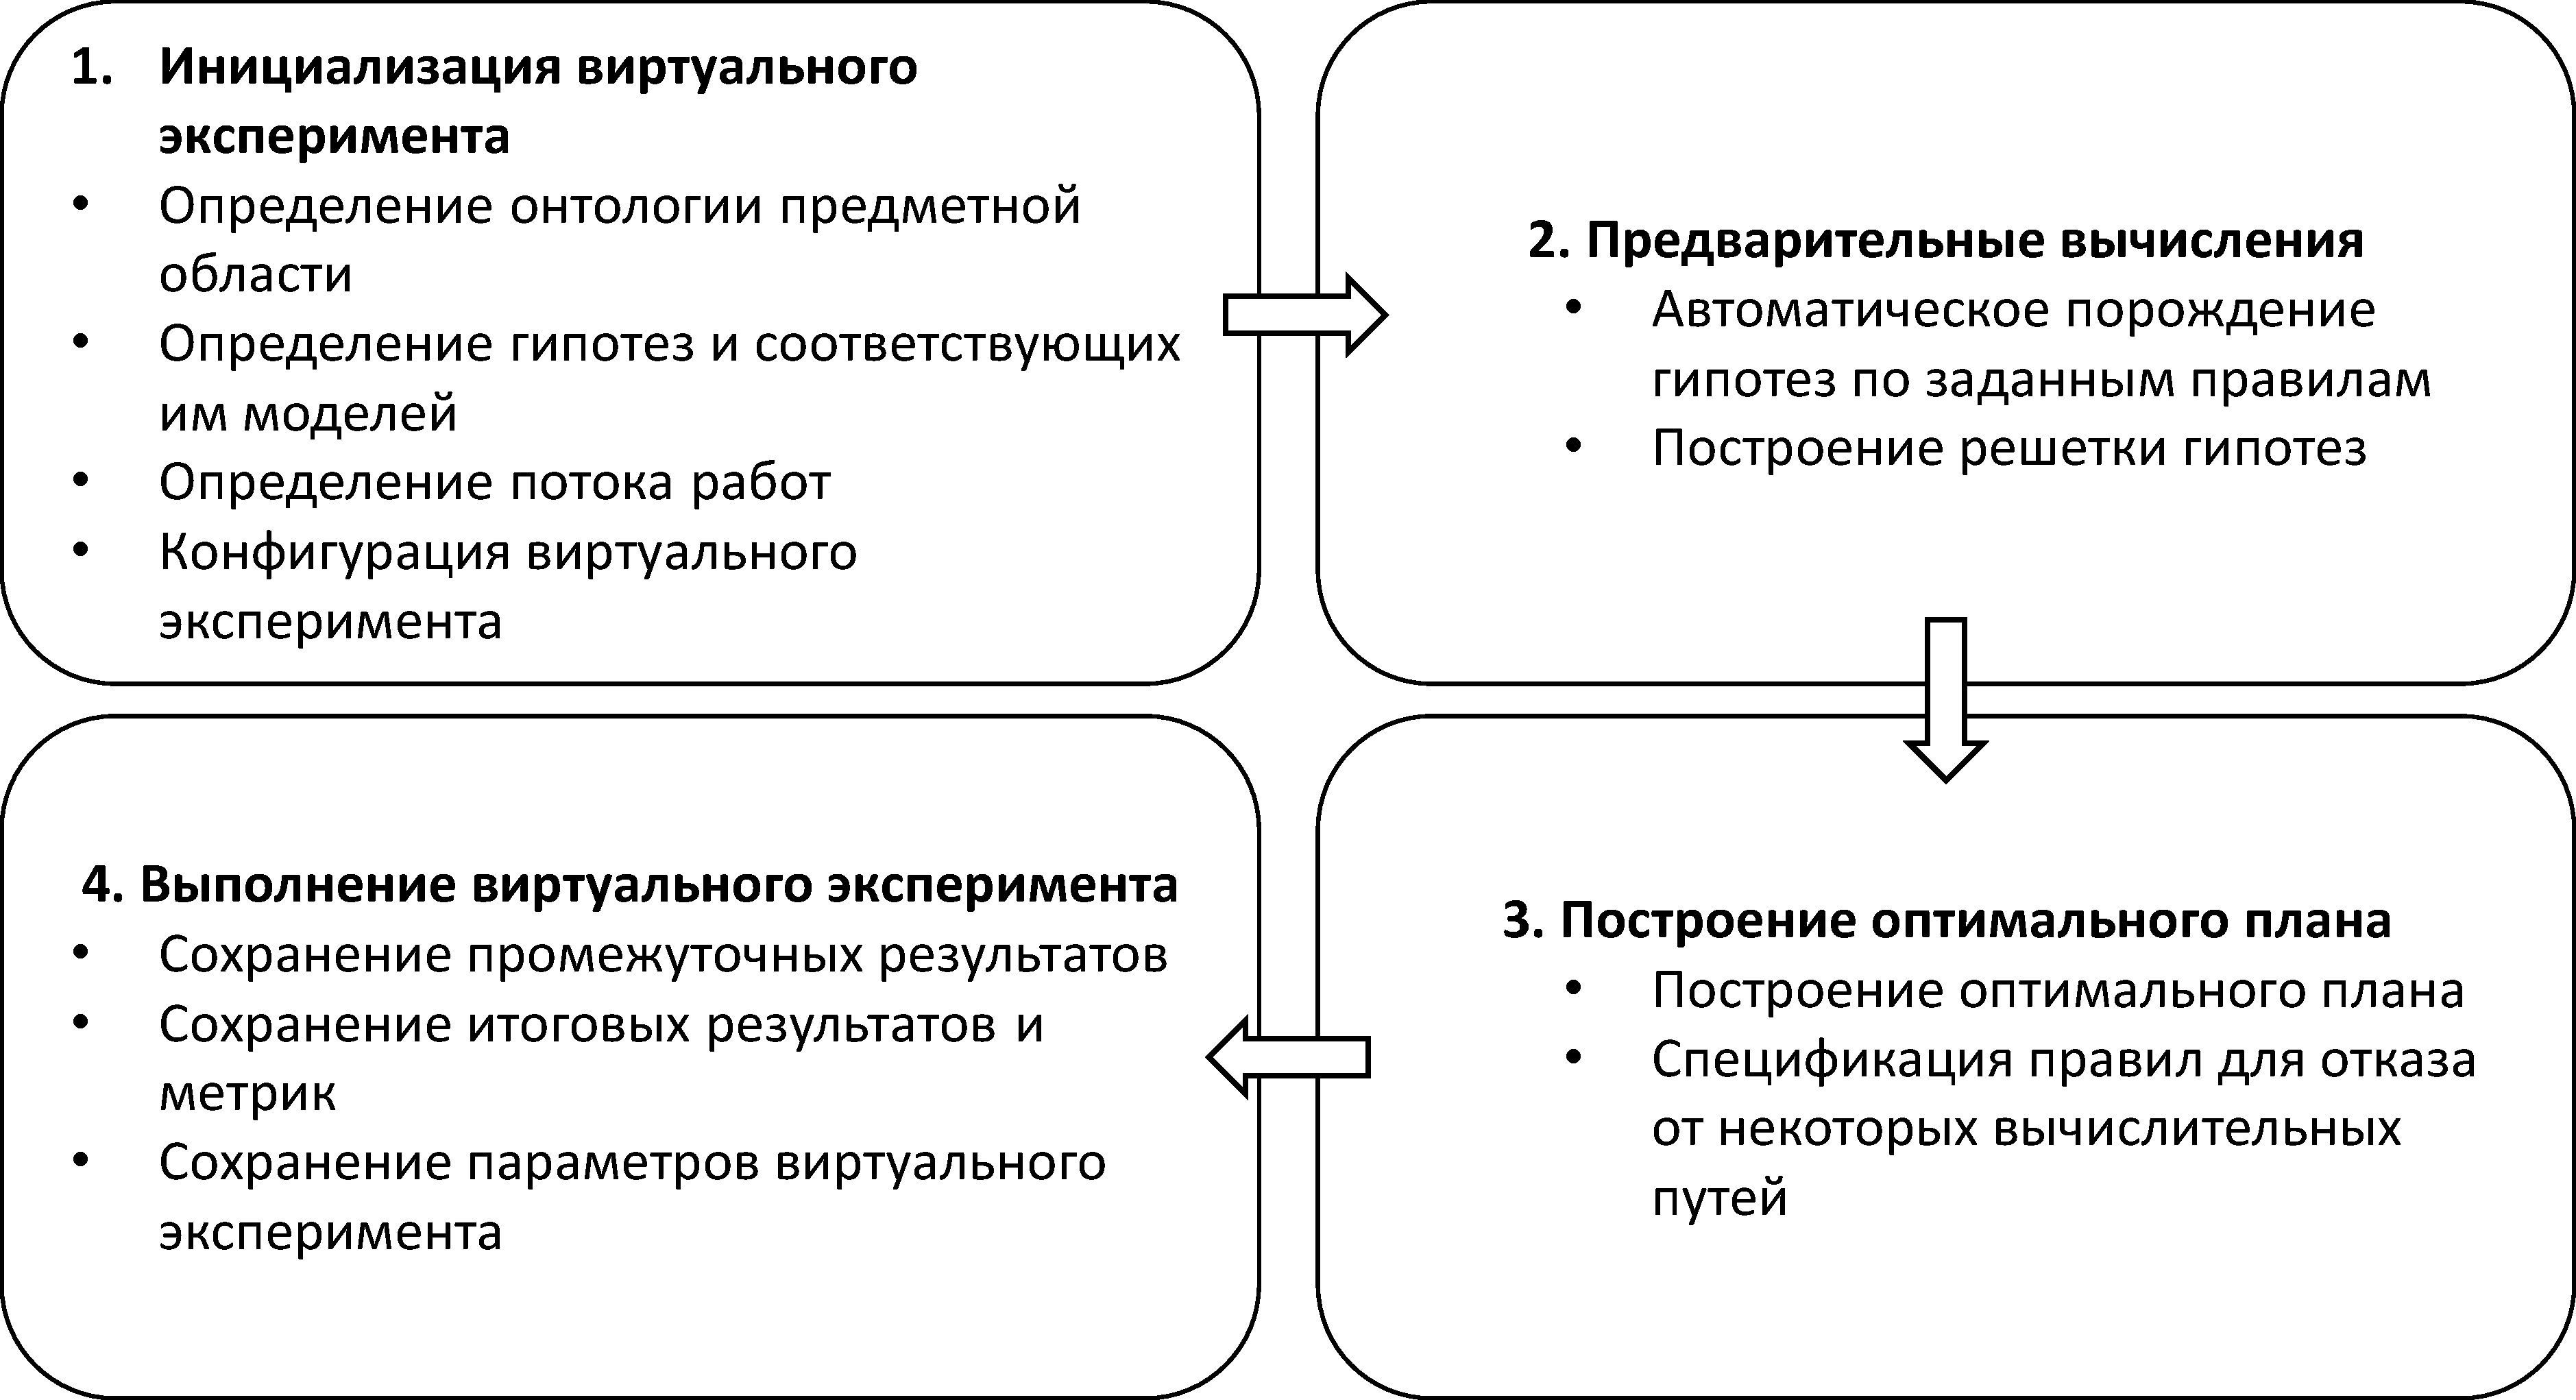
\includegraphics[width=0.9\linewidth]{images/ve_cycle.pdf}
    \caption{Жизненный цикл виртуального эксперимента.}\label{fig:lifecycle_ve}
\end{figure}


На первом этапе происходит инициализация виртуального эксперимента: определение онтологии предметной области, 
определение гипотез и соответствующих им моделей, определение потока работ для исполнения виртуального эксперимента, 
задание конфигурации эксперимента. Поток работ также определяется как направленный ациклический граф. Вершины такого 
графа называются задачами, а каждая задача рассматривается как программа, вызывающая функции, реализующие гипотезы.

На втором этапе по желанию пользователя происходит автоматическое порождение дополнительных гипотез из данных. 
После загрузки виртуального эксперимента в систему происходит автоматическое построение решетки гипотез виртуального 
эксперимента. Используется представление гипотез как специальных структур данных, сочетающих равенства, входящие в 
них переменные и причинно-следственные отображения над ними. Решетка гипотез определяется как направленный ациклический 
граф с вершинами, отвечающими гипотезам. Ребра графа соответствуют отношению завимости между гипотезами, когда 
результат вычислений одной гипотезы используется в вычислениях другой гипотезы. Конструирование решеток отношений 
между гипотезами способствует повышению эффективности управления виртуальными экспериментами, в частности, ускорению 
вычислений с использованием промежуточных результатов, относящихся к независимым гипотезам. 

На третьем этапе происходит построение оптимального плана исполнения нескольких экспериментов. 

На четвертом этапе происходит непосредственное исполнение одного или нескольких виртуальных экспериментов, при этом 
система отслеживает, есть ли в базе данных метаинформации сохраненные результаты исполнения отдельных функций 
эксперимента при заданных параметрах и подставляет их, если совпадение найдено. После исполнения виртуального 
эксперимента результат возвращается эксперту.

Далее предствален алгоритм построения решетки гипотез. 
\textit{Определение 2.} Решетка гипотез $L$ представляет собой ориентированный ациклический граф, вершины которого 
соответствуют гипотезам с некоторой структурой $S$, а ребра соответствуют отношению $derived\_by$  между гипотезами. 
Отношение $derived\_ by\left(b, a\right)$ означает, что результат вычисления гипотезы $b$ используется при вычислении 
гипотезы $a$.

Разработанный алгоритм построения решетки гипотез в виртуальных экспериментах представлен в алгоритме
\ref{alg:build_lattice}. На входе алгоритм принимает поток работ $W$ и набор гипотез $H$. 
Если поток работ ссылается на гипотезу, которая не представлена в $H$, алгоритм возвращает ошибку. 
В противном случае возвращается решетка гипотезы $L$.  

Задачи потока работ рассматриваются одна за другой в соответствии с порядком, определяемым направлением ребер. 
Для каждой пары гипотез $h_i, h_j$, где $h_i$ упоминается в текущей задаче, а $h_j$ упоминается в некоторой задаче, 
достижимой из текущей задачи, строится транзитивное замыкание для объединения структур соответствующих гипотез. 
После этого все такие транзитивные замыкания объединяются вместе в $C^+$. Структура результирующей решетки $L$ 
соответствует структуре $C^+$. В качестве вершин $L$ включает гипотезы, в которых встречаются переменные из $C^+$. 
Для каждой пары $\left(x_a, x_b\right)$ в $C^+$ \textit{L} включает ребро 
$derived\_by \left(\phi^{-1}\left(x_b\right), \phi^{-1}\left(x_a\right)\right)$.

\begin{algorithm}
    % \SetKwFunction{isOddNumber}{isOddNumber}
    % \SetKwInput{Input}{Input}
    % \SetKwInput{Output}{Output}
    % \SetKwInOut{KwIn}{Input}
    % \SetKwInOut{KwOut}{Output}


    \KwIn{$W$ "--- \texttt{поток работ}, $H$ "--- \texttt{гипотезы}.}
    \KwOut{$L$ "--- \texttt{решетка гипотез}.}

    \For{$h \in V(W)$}{
        \If{$h \notin H$}{
            \textbf{вернуть} \texttt{'Ошибка: гипотезы не найдены'} 
        }
    }
    
    $ C^+ \gets \varnothing $ 

    $\phi \gets \varnothing $ 

    $L \gets \varnothing $

    $ T \gets V\left(W\right) $

    \For{$t \in T$}{
        $T \gets T \setminus t$

        \For{$h_i \in t$}{
            \For{$remain\_t$ \texttt{в} $T$, \texttt{таких что} $remain\_t$ \texttt{достижим из $t$}}{
                \For{$h_i \in remain\_t$}{
                    $S_i \gets $ \texttt{структура для } $h_i$
                    
                    $S_j \gets $ \texttt{структура для } $h_j$
                    
                    \If{$S_i \cup S_{j}$ "--- \texttt{полная}}{ 
                        \texttt{построить транзитивное замыкание } $C_{ij}^+$ \texttt{для} $S_i \cup S_{j}$
                        $C^+ \gets C^+ \cup C_{i}^+ $
                    }
                }
            }
        }
    }

    $\phi \gets $ \texttt{полное причинно-следственное отображение для} $C^+$
    
    $ L \gets L_{inp}$ 
    \For{\texttt{пара} $\left( x_a, x_b \right) \in C^+$}{
    $ V\left(L\right) \gets V\left(L\right) \cup \{\phi^{-1} \left(x_a\right)\}
             \cup \{\phi^{-1} \left(x_b\right)\}$
    
    $ E \left(L\right) \gets E\left(L\right) \cup \{ derived\_by \left(\phi^{-1} \left(x_b\right), 
    \phi^{-1} \left(x_a\right) \right) \} $
    }

    \KwRet{$L$}
    \caption{Построение решетки гипотез}\label{alg:build_lattice}
\end{algorithm}

\textbf{Лемма 1.} Вычислительная сложность алгоритма построения решетки гипотез для потока работ $W$ и набора гипотез 
$H$ ограничена функцией $ O\left( |W|^2 * |S| * |V| * |H| \right)$, где 
$S = \bigcup\limits_{h \in H} S\left(E_h, V_h \right), V = \bigcup\limits_{h \in H} V_h$.

\textbf{Доказательство.} Самой вычислительно сложной операцией алгоритма является построение транзитивного замыкания. 
Так как алгоритм состоит из трех циклов, то максимальное количество операций транзитивного замыкания не превосходит 
$|W|^2*|H|$, где $|H|$ "--- общее количество гипотез. Сложность построения транзитивного замыкания не превосходит 
$O\left(|S|*|V|\right)$, поэтому вычислительная сложность алгоритма построения решетки гипотез ограничена 
$O\left(|W|^2*|H|*|S|*|V|\right)$.

Аналогично представлен алгоритм добавления новой гипотезы в существующую решетку.

Для корректного запуска виртуальный эксперимент должен быть \textit{непротиворечивым}. 
Для этого должны выполняться следующие условия:
\begin{enumerate}
    \item Должны быть опредены все элементы виртуального эксперимента $O, H, M, R, W, C$.
    \item Число гипотез должно быть не менее числа задач в потоке работ $|H| \geq |V(W)| $.
    \item Число моделей должно быть не менее числа гипотез $|M| \geq |H|$.
    \item Для каждой гипотезы должна быть опредена реализующая ее модель: $ \forall h \in H: \exists m \in M$ такой, 
            что $h \rightarrow m \in R$.
    
    \item Для каждой задачи потока работ должен существовать набор значений параметров вызываемых функций 
            $ \forall t \in V(W): \exists c \in C$.
    \item После построения решетки гипотез запускается алгоритм \ref{alg:consistence} проверки отсутствия 
            некорректных зависимостей гипотез в потоке работ.
\end{enumerate}

Если нарушено условие 1), то платформа не сможет запустить выполнение виртуального эксперимента.
При нарушении условия 2) у некоторых задач потока работ будут отсутствовать соответствующие им гипотезы, что не 
позволит корректно построить решетку гипотез. При нарушении условия 3) и 4) некоторым гипотезам не будут 
сопоставлены модели, следовательно их будут невозможно исполнить. Условие 5) гарантирует, что для каждой модели 
существуют параметры ее запуска. Условие 6) необходимо для избежания циклов в графе потока работ, что приведет к 
некорректному построению решетки гипотез. Если гипотеза используется в задаче потока работ, то она не может быть 
использована в других задач, достижимых из этой. 

В алгоритме \ref{alg:plan} представлено построение плана виртуального эксперимента. На вход алгоритм принимает 
конфигурацию эксперимента, решетку гипотез, а на выходе возвращает два набора гипотез, модели для которых требуют или 
не требуют пересчета.



\begin{algorithm}
    \SetKwFunction{isOddNumber}{isOddNumber}
    % \SetKwInput{Input}{Input}
    % \SetKwInput{Output}{Output}
    % \SetKwInOut{KwIn}{Input}
    % \SetKwInOut{KwOut}{Output}

    \KwIn{$C$ "--- \texttt{конфигурация эксперимента}, $L$ "--- \texttt{решетка гипотез}.}
    \KwOut{$P_{ne}$ "--- \texttt{множество гипотез, для которых требуется пересчитать модели}, 
           $P_{e}$ "--- \texttt{прочие.}}

    $L_{n} \gets $ ближайшая для $L$ решетка в репозитории данных

    $P_{ne} \gets \varnothing , P_{e} \gets \varnothing $ 

    $F \gets \varnothing $

    $V \gets V(L_n)$

    % DFS 
    \For{$h \in V$}{ \Comment{начало с самой верхней гипотезы}
        \If{$\forall c_m \in C, \forall m \in M \  \alpha \  s.t.\  \nexists h \to m(c_m)$}{
            \Comment{в репозитории нет вычисленной части эксперимента}
            $H_{dep} \gets $ все зависимые гипотезы от $h$
            
            $P_{ne} \gets P_{ne}  \cup H_{dep} \cup h$

            $F \gets F \cup H_{dep} \cup h$
        }
        \Else{
            \Comment{в репозитории есть вычисленный фрагмент}

            $P_{e} \gets P_{e} \cup h$

            $F \gets F \cup h$
        }
        
        $V \gets V \setminus F $
    }
        
    \KwRet{$P_{ne}, P_{e}$}
    \caption{Построение плана виртуального эксперимента}\label{alg:plan}
\end{algorithm}

Сначала ищется ближайщая решетка, которая уже была вычисленна. После этого происходит поиск в глубину, начиная с 
гипотезы, у которой нет входных ребер. Если для всех параметров из конфигурации, для всех моделей не существует 
реализации гипотезы, то тогда гипотеза не имеет соответствующей вычисленной части и требует вычисления. Также 
требуется пересчитать модели, соответствующие всем зависимым гипотезам. Все вершины с этими гипотезами 
не требуется обходить. Иначе можно не пересчитывать соответствующий фрагмент и перейти к следующей вершине. 

Дополнительно могут быть определены эвристики для отказа от вычислительных маршрутов. Например, такой эвристикой может 
быть следующая: если коэффициент детерминации модели, реализующей гипотезу, не достигает 0.7, то требуется прекратить
вычисления и отказаться от этого вычислительного маршрута.

\begin{algorithm}
    \SetKwFunction{isOddNumber}{isOddNumber}
    % \SetKwInput{Input}{Input}
    % \SetKwInput{Output}{Output}
    % \SetKwInOut{KwIn}{Input}
    % \SetKwInOut{KwOut}{Output}

    \KwIn{$W$ "--- \texttt{поток работ}, $L_{inp}$ "--- \texttt{решетка гипотез}.}
    \KwOut{\textit{True} "--- \texttt{некорректные зависимости отсутствуют,} \textit{False} "--- \texttt{иначе}.}

    \textit{correct} $\gets$ \textit{True}

    \For{$t \in V(W)$}{  \Comment{задачи перебираются последовательно}

        \For{$h \in t$}{\Comment{проверяются все гипотезы из задачи}
            \texttt{найти все зависимые $\{h_d\} \in V(L_{inp})$ от $h$ }
            
            \For{\texttt{$remaining\_task$ достижимых из $t$}}{

                \If{$\{h_d\} \cap H_t \neq \emptyset\  \alpha\  s.t.\  H_t \in remaining\_task$}{
                    \Comment{Эксперимент определен некорректно}

                    correct $\gets$ \textit{False}   
                }
            }
        }
    }
    \KwRet{correct}
    \caption{Проверка отсутствия некорректных зависимостей гипотез в потоке работ}\label{alg:consistence}
\end{algorithm}

Отдельно определен отдельный ядровой модуль, содержащий классы, соответствующие ключевым понятиям, используемым при работе 
с платформой "--- виртуальный эксперимент, гипотеза, модель, поток работ, конфигурация. Дополнительно определены 
вспомогательные классы переменной, уравнения, структуры, решетки гипотез, полного причинно-следственного отображения, 
множества зависимых переменных и их транзитивного замыкания. 


\underline{\textbf{Третья глава}} посвящена исследованию платформы (\cref{fig:arch}) проведения виртуального 
эксперимента и то, каким образом компоненты архитектуры поддерживают различные этапы деятельности эксперта 
по проведению виртуальных экспериментов. На рисунке пунктирные стрелки обозначают доступ из одного компонента к интерфейсу другого компонента. Программная 
архитектура системы исполнения виртуального эксперимента включает в себя компоненты, поддерживающие различные этапы 
проведения виртуальных экспериментов. В настоящее время архитектура находится в стадии программной реализации.

\begin{figure}[h!]
    \centering
    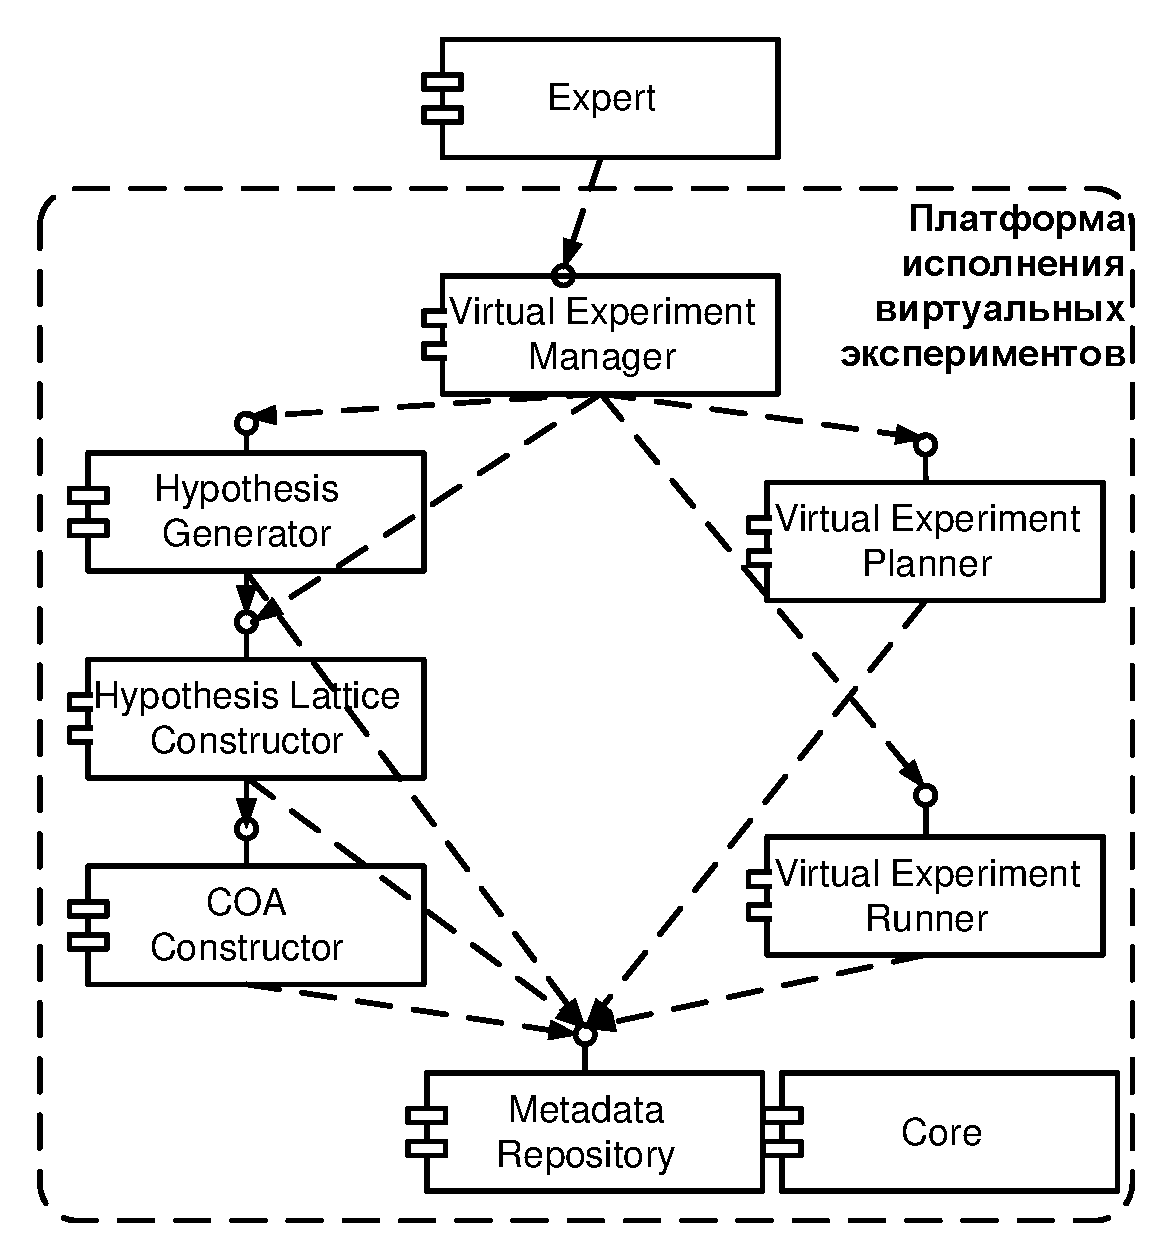
\includegraphics[width=0.7\linewidth]{images/arch_v4.pdf}
    \caption{Архитектура платформы исполнения виртуальных экспериментов.}\label{fig:arch}
\end{figure}


Разработанный в рамках проекта прототип системы управления виртуальными экспериментами нацелен на объединение 
преимуществ и преодоление недостатков существующих систем. На основании анализа предметной области управления 
виртуальными экспериментами и родственных работ формализовано общее понятие виртуального эксперимента, включающее 
онтологию предметной области, набор спецификаций гипотез и взаимосвязей между ними, набор моделей, реализующих 
гипотезы, поток работ, реализующий эксперимент, конфигурацию (набор значений параметров) эксперимента. Сформулированы 
общие требования к системе для управления виртуальными экспериментами, которым удовлетворяет реализованный прототип. 
Отслеживается эволюция моделей, гипотез и экспериментов. На основании анализа методов формального манипулирования 
виртуальными экспериментами и гипотезами при сохранении непротиворечивости экспериментов для систем с явным 
представлением и использованием гипотез выбраны и реализованы операции управления виртуальными экспериментами и 
их составляющими (гипотезы, модели, их конфигурации). Реализованы методы ранжирования конкурирующих гипотез по 
соответствию наблюдаемым данным на одном или нескольких наборах данных. Предоставляются структуры для хранения 
результатов предыдущих экспериментов, и обеспечиваются запросы к ним. Реализован метод автоматизированного построения 
решеток причинно-следственных зависимостей гипотез в виртуальных экспериментах. Реализован метод порождения гипотез 
из данных, сочетающий обобщенную линейную модель, генетическое программирование и динамическое причинно-следственное 
моделирование. Разработаны и реализованы метод поиска оптимальных параметров гипотез и метод корректной оценки 
соответствия гипотезы исследуемому явлению. Реализован метод повышения эффективности и скорости проведения виртуальных 
экспериментов. Реализованы методы сравнения конкурирующих гипотез, построенных из данных, с теоретическими гипотезами 
из теоретического моделирования или литературы. Реализован подход к интеграции экспериментов, гипотез и данных с 
данными новых наблюдений, симуляций и метаданных экспериментов.

Компонент MetadataRepository представляет собой репозиторий метаинформации (базу данных), предназначенный для хранения 
результатов выполнения виртуального эксперимента с учетом накопления данных о добавлении, модификации и удалении 
гипотез, потоков работ, онтологий и виртуальных экспериментов. Дополнительно в репозитории сохраняются построенные 
зависимости между гипотезами (полученными либо от эксперта, либо автоматически извлеченные) и имеющейся информации 
о корреляции между параметрами как в рамках одной, так и параметров нескольких гипотез.

Компонент VirtualExperimentManager представляет пользователю интерфейс с операциями формального манипулирования 
виртуальными экспериментами и гипотезами. После загрузки виртуального эксперимента в систему его спецификация 
сохраняется в базу данных. Далее, по запросу эксперта происходит вызов компонента автоматического порождения 
гипотез из данных HypothesisGenerator. После этого автоматически происходит вызов компонента 
HypothesisLatticesConstructor для построения решетки гипотез виртуального эксперимента. Далее вызывается компонент 
VirtualExperimentPlanner, отвечающий за построение плана исполнения виртуального эксперимента. Построенный план 
сохраняется в базу данных. Наконец, происходит вызов компонента VirtualExperimentRunner, ответственного за 
непосредственное исполнение виртуального эксперимента. Компонент поддерживает одновременное управление 
несколькими экспериментами.

На основании проведенного анализа существующих методов предложен метод порождения гипотез из данных. Основные 
положения метода состоят в следующем. Сначала над данными запускается метод GLM, в результате работы которого 
выделяются такие комбинации переменных, коэффициент при которых значимо отличен от нуля. Одновременно с GLM, для
 этого же набора данных выполняется метод динамического причинно-следственного моделирования. Из полученной для 
 DCM системы уравнений извлекаются только производные от переменных. Далее комбинации переменных GLM и производные 
 переменных метода DCM используются в качестве входных данных для метода генетического программирования. 
 Использование подобной эвристики позволяет значительно сократить время работы метода, при этом увеличивается 
 точность соответствия данным наблюдений. Параллельно запускается метод подбора функции в неявном виде с использованием 
 нейронных обыкновенных дифференциальных уравнений. Вычисленные системы уравнений ранжируются с использованием 
 метрики "--- коэффициента детерминации, эксперту возвращается функция с наибольшей метрикой. При необходимости 
 эксперт может получить формулу зависимости в явном или неявном виде.

Компонент HypothesisGenerator по запросу эксперта обеспечивает автоматическое построение гипотез по данным в виде 
нелинейных функциональных зависимостей. В качестве основного метода используется символьная регрессия, обеспечивающая 
интерпретируемость полученных формул. Эксперту вместе с системой уравнений возвращается оценка качества соответствия 
данным, по которой принимается решение об использовании построенной гипотезы. Компонент реализован в виде модуля на 
языке Python с использованием библиотек pandas, numpy, sympy, deap [5]. Для построения функциональной зависимости 
между переменными в данных используется реализация символьной регрессии на основе генетического программирования 
с арифметическими и тригонометрическими операциями [7]. 

Компонент COAConstructor позволяет построить причинно-следственный граф зависимостей переменных одной гипотезы. 
Компонент включает механизм вероятностного вывода, позволяющего отследить не только причинно-следственные связи между 
гипотезами, но и неявные зависимости, например, значимые корреляции между параметрами гипотез, не связанных 
причинно-следственными зависимостями. Использование пар значимо коррелирующих переменных позволяет системе указывать 
эксперту, например, на необходимость их совместного изменения. Компонент реализован в виде модуля на языке Python 
с использованием библиотек numpy, latex2sympy, owlready, graphviz, sympy, networkx. Диаграмма классов компонента 
приведена на \cref{fig:base_coa}.

\begin{figure}[h!]
    \centering
    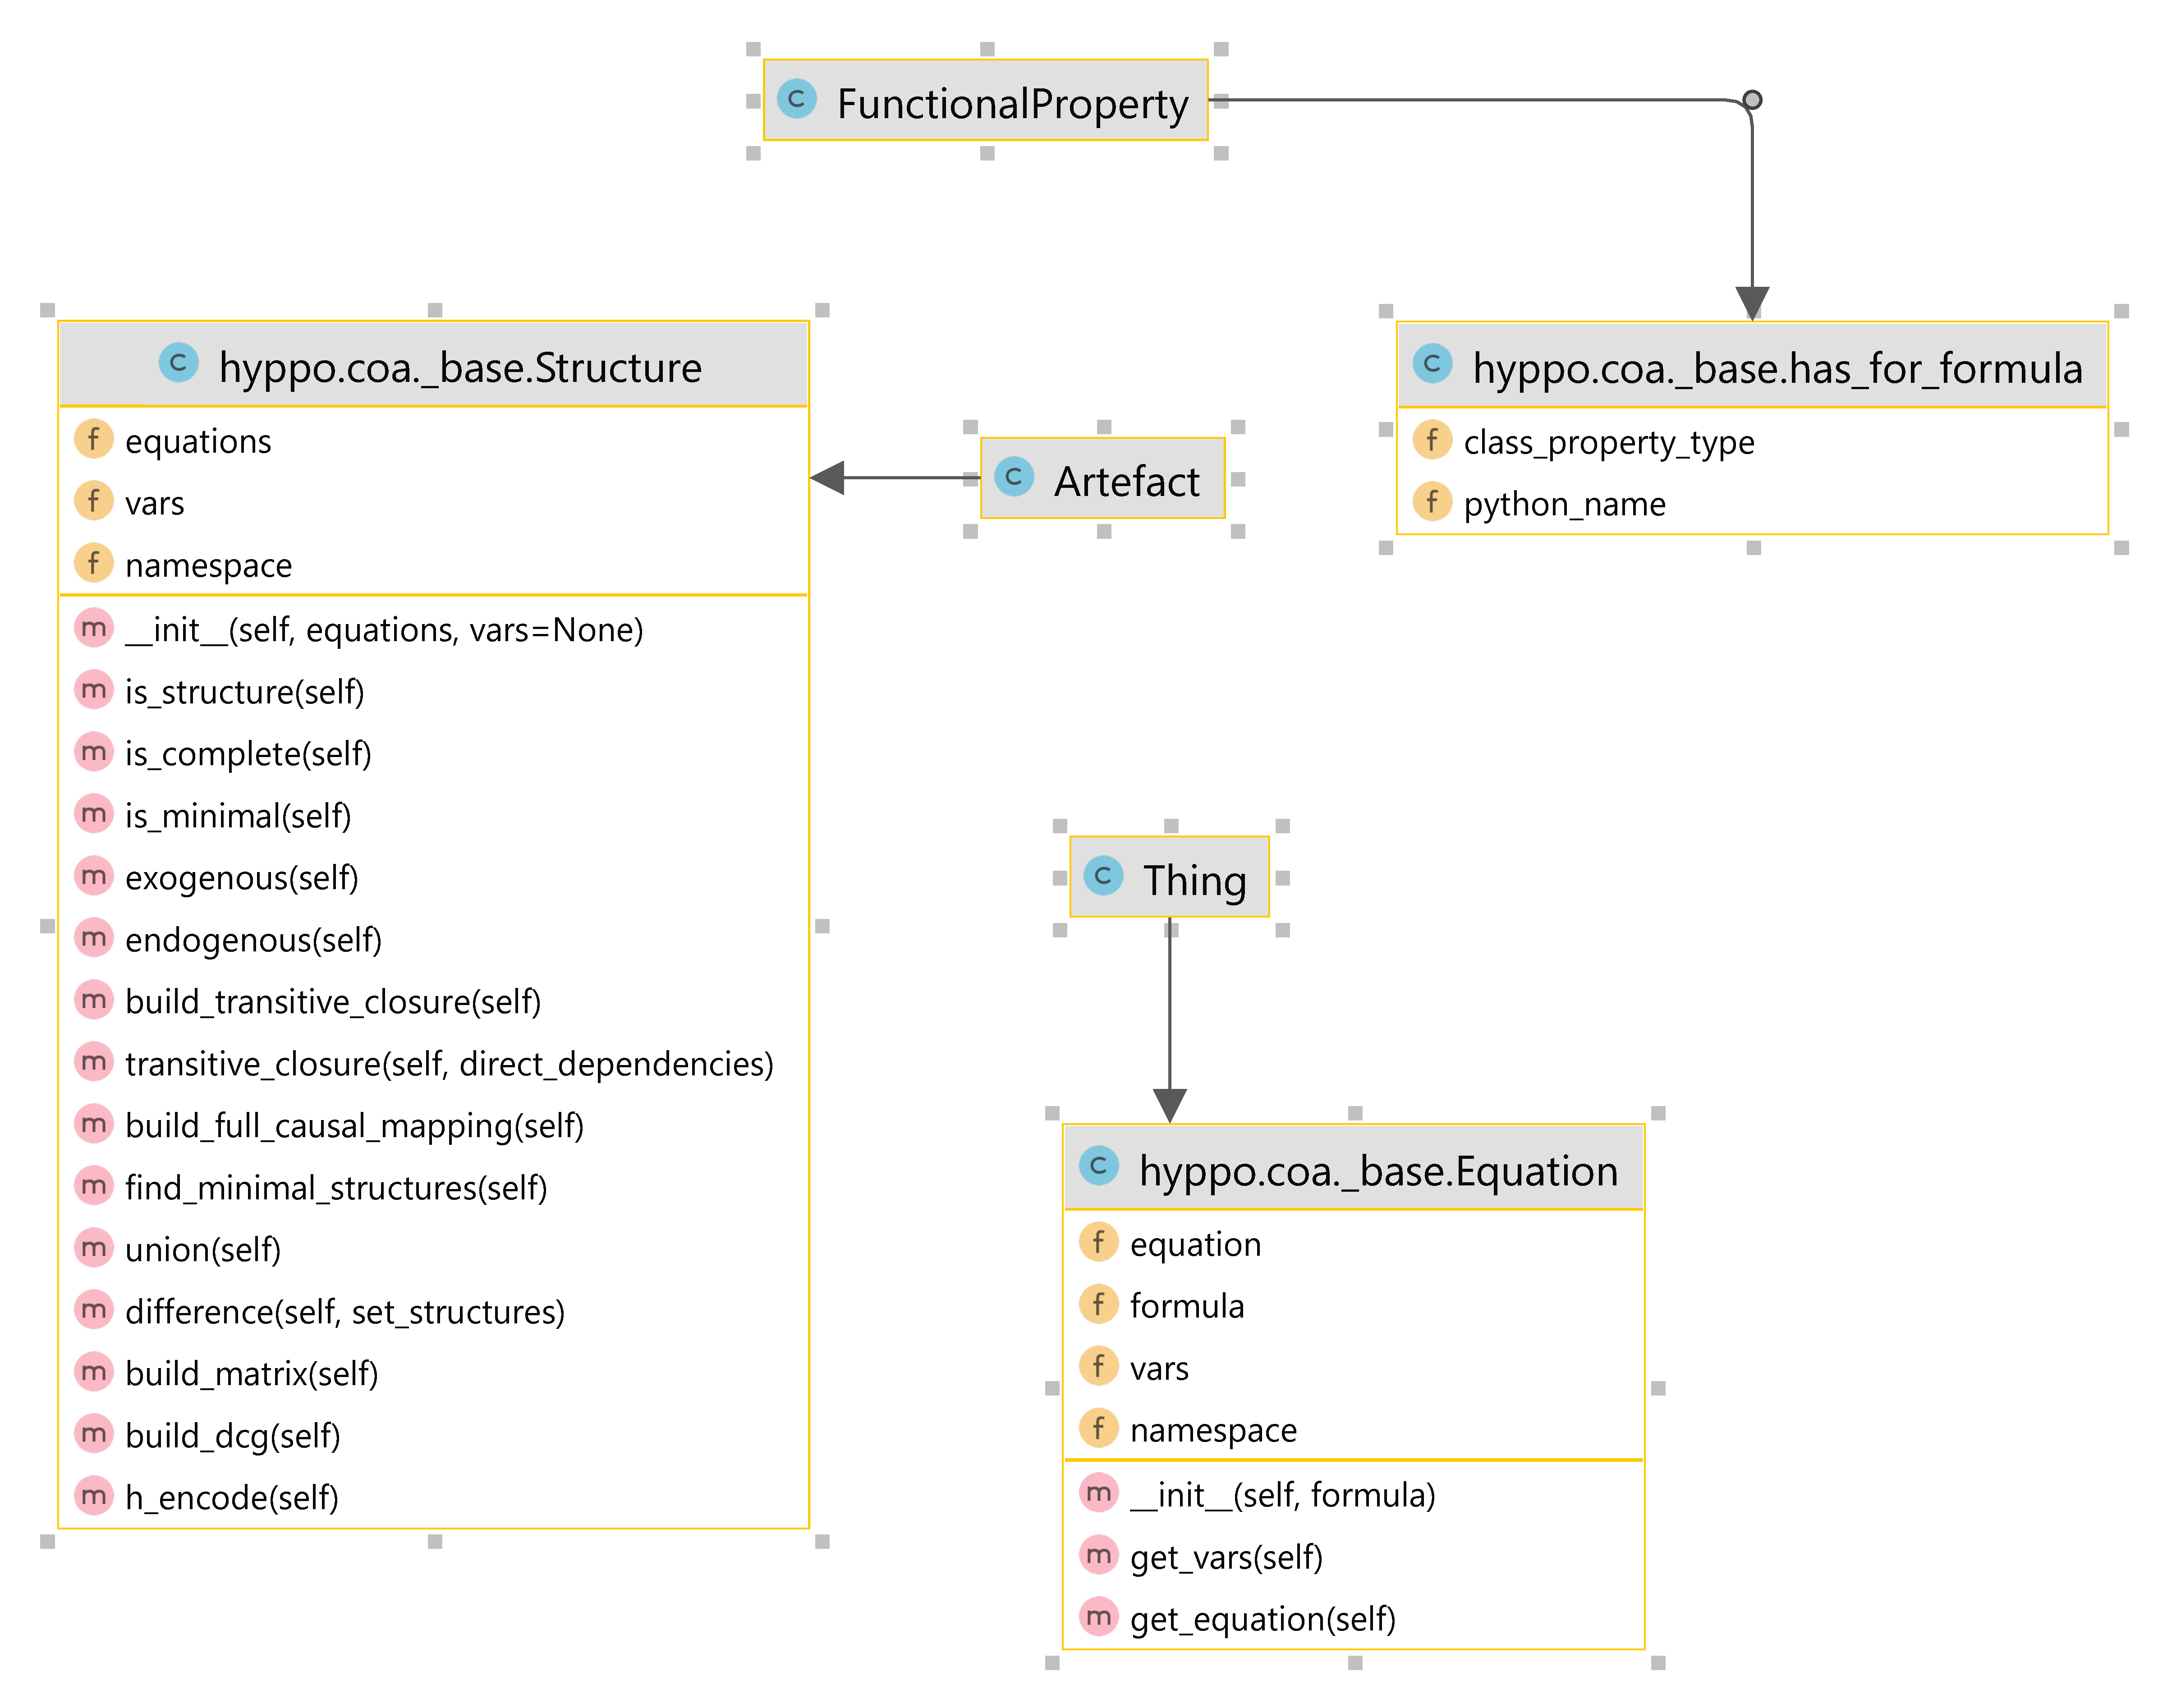
\includegraphics[width=0.9\linewidth]{images/base_coa.pdf}
    \caption{Диаграмма для пакета.}\label{fig:base_coa}
\end{figure}


Компонент HypothesisLatticesConstructor обеспечивает автоматическое построение решеток гипотез по соответствующим 
им системам уравнений. Компонент загружает из базы данных метаинформации спецификацию потока работ и гипотез. 
Далее системы уравнений, соответствующих гипотезам, из спецификации переводятся во внутреннее представление, 
после чего вызывается компонент COAConstructor для построения причинно-следственного графа зависимостей переменных. 
Решетка гипотез сохраняется в базу данных метаинформации. Компонент реализован в виде модуля на языке Python с 
использованием библиотек pandas, numpy, itertools.

Разработанный метод построения решеток гипотез реализован в виде отдельного компонента на языке Python 3.6 с 
использованием библиотеки для научных вычислений scipy и библиотеки поддержки многомерных массивов numpy. Компонент 
включает в себя функции загрузки спецификаций потока работ и гипотез, построения решетки гипотез по набору гипотез и 
потоку работ, вывод и сохранение результатов в локальную файловую систему. Входными данными для алгоритма являются 
спецификации потока работ и гипотез, загружаемые из локальной файловой системы. Реализация алгоритма построения 
решеток гипотез выполнена в отдельной функции, сохранение и отображение решетки гипотез также выполнено 
в отдельной функции.

Основная идея метода повышения эффективности и скорости проведения виртуальных экспериментов состоит в следующем. 
На вход метод принимает спецификацию виртуального эксперимента и построенную для него решетку гипотез. Из множества 
гипотез виртуального эксперимента извлекаются конкурирующие гипотезы, т.е. те, для которых существует несколько 
возможных значений их параметров (гипотезы с разным значением одного параметра конкурируют друг с другом). 
Составляется сетка всевозможных комбинаций таких параметров. Далее с использованием решетки гипотез определяется 
порядок подстановки построенных комбинаций параметров в процессе исполнения виртуальных экспериментов. 
Данный процесс происходит итеративно, при этом на каждом шаге из решетки гипотез убираются гипотезы, не имеющие 
зависящих от себя других гипотез. Если для таких гипотез существуют конкурирующие, то подобная конфигурация 
параметров добавляется в план исполнения виртуального эксперимента. При этом те вызовы функций моделей, параметры для 
которых не изменились, считаются не требующими повторного вычисления, т.е. при непосредственном исполнении 
подставляется уже вычисленный фрагмент виртуального эксперимента. На выходе предоставляется план исполнения 
виртуального эксперимента с указанием порядка подстановки комбинаций параметров, а также частей виртуального 
эксперимента, требующих вызова функций моделей с новыми параметрами.

Метод применим как для работы с новым виртуальным экспериментом, так и для модифицированного виртуального 
эксперимента, например, после добавления в него нового значения параметров для существующей гипотезы. В первом 
случае будет возвращен план исполнения для всего эксперимента, тогда как во втором - только для новых комбинаций 
параметров. При изменении решетки гипотез или спецификации виртуального эксперимента данный метод в системе управления 
виртуальными экспериментами следует вызывать автоматически.
Алгоритм, реализующий разработанный метод, выполнен на языке Python 3.6 с использованием библиотек NumPy, SciPy, 
Pandas. Реализация выполнена в виде отдельного модуля. Для хранения результатов проведенных экспериментов используется 
реляционная база данных.


Компонент VirtualExperimentRunner запускается для непосредственного исполнения виртуального эксперимента. 
Из репозитория метаинформации загружаются спецификация виртуального эксперимента и дополнительно построенные 
решетка гипотез и план исполнения виртуального эксперимента. Исполнение происходит в соответствии с планом, при 
этом система использует сохраненные результаты исполнения части виртуального эксперимента (при их наличии в 
репозитории метаинформации). Используя спецификацию моделей виртуального эксперимента, компонент осуществляет 
вызов соответствующих функций, а затем собирает полученные данные от них. Результаты исполнения виртуального 
эксперимента сохраняются в базу данных метаинформации.

Эксперименты по адаптации программной реализации нейросетевых моделей для выполнения в распределенной 
вычислительной среде были проведены с использованием прототипа вычислительного кластера. Кластер включает в 
себя главный узел и четыре вычислительных узла и развернут как часть инфраструктуры совместных исследовательских 
объектов для высокопроизводительных вычислений ФИЦ ИУ РАН. Аппаратная архитектура кластера показана на 
\cref{fig:lab_cluster}. Вычислительные узлы включают в себя два процессора Intel Xeon 2630L с частотой 2,5 ГГц и 
24 виртуальными ядрами, 64 ГБ оперативной памяти DDR3 1066 МГц, один твердотельный накопитель емкостью 160 Гб и 
четыре жестких диска емкостью 2 ТБ каждый. Кластер также включает файловый сервер Quanta Stratos S810 с двумя 
процессорами Intel XEON 2670, 96 ГБ оперативной памяти DDR3 1066 МГц, один твердотельный накопитель INTEL S3500 
емкостью 480 ГБ, RAID-массив, состоящий из 15 жестких дисков по 2 ТБ каждый, и RAID-массив, состоящий из 
8 твердотельных накопителей INTEL S3500 емкостью 480 ГБ каждый. Сеть Ethernet поддерживается коммутатором 
Quanta LB6M 10GbE.


\begin{figure}[h!]
    \centering
    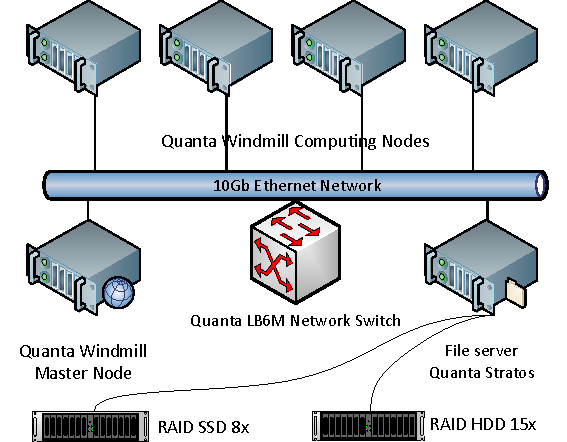
\includegraphics[width=0.7\linewidth]{images/lab_cluster.pdf}
    \caption{Инфраструктура платформы исполнения виртуальных экспериментов.}\label{fig:lab_cluster}
\end{figure}

В \underline{\textbf{четвертой главе}} приведено описание

\FloatBarrier
\pdfbookmark{Заключение}{conclusion}                                  % Закладка pdf
В \underline{\textbf{заключении}} приведены основные результаты работы, которые заключаются в следующем:
%% Согласно ГОСТ Р 7.0.11-2011:
%% 5.3.3 В заключении диссертации излагают итоги выполненного исследования, рекомендации, перспективы дальнейшей разработки темы.
%% 9.2.3 В заключении автореферата диссертации излагают итоги данного исследования, рекомендации и перспективы дальнейшей разработки темы.
\begin{enumerate}
  \item Проведен анализ существующих средств концептуального моделирования гипотез в процессе проведения виртуальных экспериментов. На основе анализа \ldots
  \item Осуществлена разработка методов автоматизированного построения решеток гипотез в виртуальных экспериментах. \ldots
  \item Проведена реализация метода построения решеток гипотез в виде отдельного компонента системы. \ldots
  \item Проведен анализ методов формального манипулирования виртуальными экспериментами и гипотезами при сохранении непротиворечивости экспериментов для систем с явным представлением и использованием гипотез.
  \item Проведено исследование и разработка методов автоматического порождения гипотез из данных.
  \item Разработаны метод поиска оптимальных параметров гипотез и метод корректной оценки соответствия гипотезы исследуемому явлению.
  \item Реализован метод повышения эффективности и скорости проведения виртуальных экспериментов.
  \item Применимость разработанных методов и подходов продемонстрирована на задаче из предметной области нейрофизиологии, связанной с поиском функциональной связности областей человеческого мозга над данными проекта HCP.
  \item Разработаны методы сравнения построенных из данных гипотез с теоретическими гипотезами из теоретического моделирования или литературы.
  \item Разработан программный прототип по обеспечению полного цикла работы с виртуальным экспериментом.
  
  \item Разработаны программы, реализующие конкретные виртуальные эксперименты в ОИИД. Для выполнения поставленных задач был создан \ldots
\end{enumerate}

% Поставленные задачи диссертационного исследования выполнены полностью.

% Результаты диссертации были применены в ходе выполнения научно-исследовательских работ:
% \begin{enumerate}
%     \item Методы и средства организации экспериментов в движимых гипотезами исследованиях в областях с интенсивным использованием данных Грант РФФИ 18-07-01434 (A).
% \end{enumerate}

\pdfbookmark{Литература}{bibliography}                                % Закладка pdf
При использовании пакета \verb!biblatex! список публикаций автора по теме
диссертации формируется в разделе <<\publications>>\ файла
\verb!common/characteristic.tex!  при помощи команды \verb!\nocite!

\ifdefmacro{\microtypesetup}{\microtypesetup{protrusion=false}}{} % не рекомендуется применять пакет микротипографики к автоматически генерируемому списку литературы
\urlstyle{rm}                               % ссылки URL обычным шрифтом
\ifnumequal{\value{bibliosel}}{0}{% Встроенная реализация с загрузкой файла через движок bibtex8
    \renewcommand{\bibname}{\large \bibtitleauthor}
    \nocite{*}
    \insertbiblioauthor           % Подключаем Bib-базы
    %\insertbiblioexternal   % !!! bibtex не умеет работать с несколькими библиографиями !!!
}{% Реализация пакетом biblatex через движок biber
    % Цитирования.
    %  * Порядок перечисления определяет порядок в библиографии (только внутри подраздела, если `\insertbiblioauthorgrouped`).
    %  * Если не соблюдать порядок "как для \printbibliography", нумерация в `\insertbiblioauthor` будет кривой.
    %  * Если цитировать каждый источник отдельной командой --- найти некоторые ошибки будет проще.
    %
    % authorvak
    \nocite{kovalev2020multidisciplinary}%
    \nocite{kovalev2020architecture}%
    \nocite{tirikov2021methods}%
    % %
    % %% authorwos
    % \nocite{wosbib1}%
    % %
    %% authorscopus
    \nocite{kalinichenko2015methods}%
    \nocite{kovalev2017organization}%
    \nocite{kovalev2017search}%
    \nocite{kovalev2019constructing}%
    \nocite{kovalev2019virtual}%
    \nocite{kovalev2020methods}%
    % %
    % %% authorpathent
    % \nocite{patbib1}%
    %
    %% authorprogram
    \nocite{progbib1}%
    % %
    % %% authorconf
    % \nocite{confbib1}%
    % \nocite{confbib2}%
    % %
    % %% authorother
    % \nocite{bib1}%
    % \nocite{bib2}%

    \ifnumgreater{\value{usefootcite}}{0}{
        \begin{refcontext}[labelprefix={}]
            \ifnum \value{bibgrouped}>0
                \insertbiblioauthorgrouped    % Вывод всех работ автора, сгруппированных по источникам
            \else
                \insertbiblioauthor      % Вывод всех работ автора
            \fi
        \end{refcontext}
    }{
        \ifnum \totvalue{citeexternal}>0
            \begin{refcontext}[labelprefix=A]
                \ifnum \value{bibgrouped}>0
                    \insertbiblioauthorgrouped    % Вывод всех работ автора, сгруппированных по источникам
                \else
                    \insertbiblioauthor      % Вывод всех работ автора
                \fi
            \end{refcontext}
        \else
            \ifnum \value{bibgrouped}>0
                \insertbiblioauthorgrouped    % Вывод всех работ автора, сгруппированных по источникам
            \else
                \insertbiblioauthor      % Вывод всех работ автора
            \fi
        \fi
        %  \insertbiblioauthorimportant  % Вывод наиболее значимых работ автора (определяется в файле characteristic во второй section)
        \begin{refcontext}[labelprefix={}]
            \insertbiblioexternal            % Вывод списка литературы, на которую ссылались в тексте автореферата
        \end{refcontext}
        % Невидимый библиографический список для подсчёта количества внешних публикаций
        % Используется, чтобы убрать приставку "А" у работ автора, если в автореферате нет
        % цитирований внешних источников.
        \printbibliography[heading=nobibheading, section=0, env=countexternal, keyword=biblioexternal, resetnumbers=true]%
    }
}
\ifdefmacro{\microtypesetup}{\microtypesetup{protrusion=true}}{}
\urlstyle{tt}                               % возвращаем установки шрифта ссылок URL
